\section{Das Projekt: iFMS@Salesforce}
%\section{Forschungsergebnisse}
\label{cha:result}
\begin{comment}
In Kapitel „Forschungsergebnisse“ stellen Sie die Ergebnisse ihrer Arbeit dar.
An dieser Stelle nehmen Sie noch keine Interpretation oder Erläuterung der 
Ergebnisse vor, sondern beschreiben rein deskriptiv ihre Befunde. Eine 
Auswertung findet im nachfolgenden Kapitel statt.
\end{comment}

Das entwickelte Vorgehensmodell soll nun auf ein Migrationsprojekt aus der 
Praxis angewendet werden. Dazu werden zunächst die Firma sowie die 
Rahmenbedingungen des Projektes vorgestellt. Anschließend wird exemplarisch 
eine Vision für das Projekt entwickelt.

\subsection{Beteiligte Unternehmen und das On-Premise-Produkt}
\usetikzlibrary{decorations.text}
\usetikzlibrary{calc}
\usetikzlibrary{fit}
\usetikzlibrary{shapes}
\usetikzlibrary{arrows,positioning} 
\pgfmathsetmacro{\cubex}{4}
\pgfmathsetmacro{\cubey}{2}

\definecolor{light-gray}{gray}{0.80}

\tikzset{
    %Define standard arrow tip
    >=stealth',
    %Define style for boxes
    punkt/.style={
           rectangle,
           rounded corners,
           draw=black, very thick,
           text width=8em,
           minimum height=2em,
           text centered},
    % Define arrow style
    pil/.style={
           ->,
           very thick,
           shorten <=5pt,
           shorten >=5pt,},
    Line/.style={
	dashed,
	very thick
    }
}




%\begin{document}
\begin{figure}[bh]
\begin{center}
\scalebox{1}{
\begin{tikzpicture}

\newcommand{\yOffset}{-1.9*\cubey}
\newcommand{\yOffsetLineBottom}{\yOffset + 0.35*\cubey}
\newcommand{\yOffsetTop}{-0.9*\cubey}
\newcommand{\imgWidthSmall}{0.17\textwidth}
\newcommand{\xOffsetBottom}{0.23*\textwidth}

\coordinate (RO) at (0,0);
\coordinate (LO) at (-\cubex,0);
\coordinate (RU) at (0,-\cubey);
\coordinate (LU) at (-\cubex,-\cubey);
%\draw (RO) -- (RU) -- (LU) -- (LO) -- (RO);
\node[] (reply) at (0,0) 
{
\includegraphics[width=0.45\textwidth]{images/reply.png} };


\node[] (syskoplan) at (0,\yOffset) 
{
\includegraphics[width=\imgWidthSmall]{images/syskoplan.jpg} };
\draw[Line] (0,\yOffsetTop) -- (0,\yOffsetLineBottom);


\node[] (arlanis) at (-\xOffsetBottom,\yOffset) 
{
\includegraphics[width=\imgWidthSmall]{images/arlanis.jpg} };
\draw[Line] (-\xOffsetBottom,\yOffsetTop) -- 
(-\xOffsetBottom,\yOffsetLineBottom);

\node (others) at (\xOffsetBottom,\yOffset) {\Huge{...}};
\draw[Line] (\xOffsetBottom,\yOffsetTop) -- 
(\xOffsetBottom,\yOffsetLineBottom);

\end{tikzpicture}
}
\caption{Das Reply Unternehmensnetzwerk. Eigene Grafik.}
\label{fig:reply}

\end{center}

\end{figure}



Reply ist ein an der italienischen Börse gehandeltes 
IT-Beratungsunternehmen und betrachtet sich als "`Living network"'\ aus 
hochspezialisierten Tochterunternehmen. Seit der Gründung 1996 konnte Reply 
seinen Umsatz auf über 705 Millionen Euro bei 5.245 Angestellten im Jahr 2015 
steigern. Das Netzwerk wuchs und wächst rasch: 2016 wurden bis November drei 
neue Firmen aquiriert. Zwei Tochtergesellschaften, die schon seit mehreren 
Jahren Teil von Reply sind, 
möchte ich genauer vorstellen, da ihre Unternehmensprofile das 
Migrationsprojekt in besonderem Maße beeinflussen.

Die vormalige syskoplan AG, seit dem Erwerb 2010 \pcite{}{12}{replycompprofile} 
Syskoplan Reply, ist ein Spezialist für SAP-Applikationen und 
-Plattformen \pcite{}{10}{replycompprofile} und entwickelt seit 1999 das 
integrierte Facility Management System (iFMS). iFMS verbindet die in SAP 
hinterlegten Daten mit Gebäudeplänen und versucht Prozesse rund um die 
Verwaltung von Immobilien zu unterstützen. Die gewachsene 
Java-Anwendung mit einer Client-Server-Architektur lässt sich inzwischen nur 
noch schwer um von Kunden gewünschte Funktionen erweitern. Auch die Bedienung 
über 
eine zusätzlich zu installierenden Anwendung wirkt in Zeiten, in denen Nutzer 
es gewohnt sind, auch umfangreiche Software über den Webbrowser zu bedienen, 
anachronstisch. Beide Aspekte schränken die zukünftige
Wettbewerbsfähigkeit der Software ein. 

Die ehemalige Arlanis Software AG wurde 2012 von Reply übernommen und ist 
Spezialist für Lösungen auf Basis des Cloud Anbieters Salesforce. Mit 
Salesforce lassen sich Lösungen häufig ganz ohne eigenen Code auf einer 
SaaS-Basis zusammen klicken. Ist doch Code erforderlich lässt er sich auf der 
PaaS-Plattform (Force.com und Heroku) entwickeln, wobei auf per SaaS angelegte 
Datenmodelle und Daten zugegriffen werden kann, auf die externe Anwendungen per 
Web Service zugreifen können. Mit Salesforce1 steht eine App für mobile Geräte 
zur Verfügung; jede Salesforce-Anwendung lässt sich über diese App bedienen. 

Über das Unternehmensnetzwerk von Reply sollen die Stärken beider 
Tochterunternehmen verbunden werden; mit dem Know-How im Bereich Facility 
Management und SAP soll auf Salesforce eine innovative, wettbewerbsfähige 
Anwendung geschaffen werden: iFMS@Salesforce.

Die On-Premise-Anwendung iFMS dient dem Facility Management. Mit ihr lassen 
sich Gebäude, Etagen und Räume verwalten, mieten und vermieten. Dabei werden in 
SAP hinterlegte Informationen wie Raumgrößen, Nutzungsarten, Adressen und 
Kontaktinformationen mit CAD Plänen verknüpft. Um iFMS zu nutzen, müssen 
Unternehmen einen Server bereitstellen und warten, auf dem der Serverteil der 
Anwendung läuft. Außerdem wird ein Datenbankserver benötigt, auf dem iFMS seine 
Daten speichern kann. Auf dem Rechner eines jeden Nutzers muss ebenfalls eine 
Anwendung installiert werden. Ein Screenshot aus Anwendersicht ist in Abbildung 
~\ref{fig:ifms_liegenschaftsbaum} dargestellt. Sie soll nicht im Detail erklärt 
werden, sondern nur die Art und Komplexität der Anwendung andeuten. 

\begin{figure}[!h]
\begin{center}
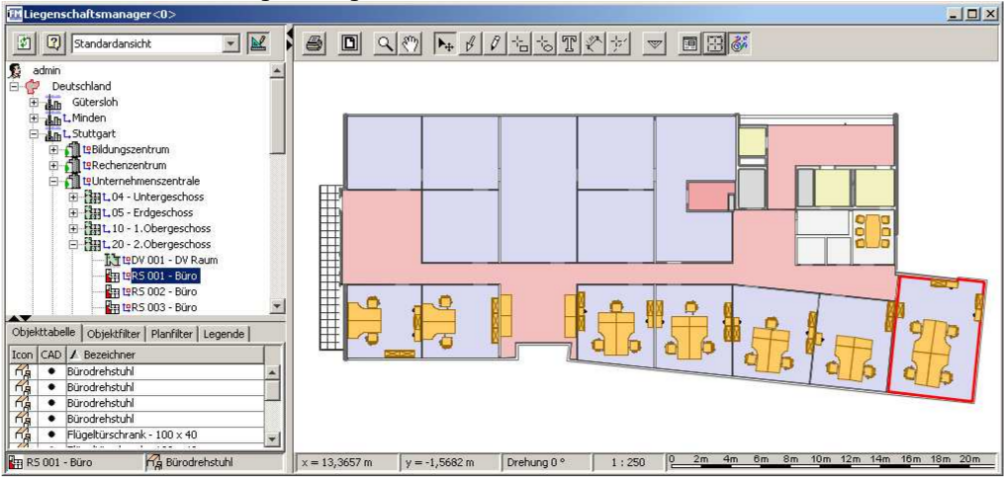
\includegraphics[width=\textwidth]{images/iFMS_liegenschaftsbaum.png}
\caption{Screenshot iFMS aus der 
Benutzerdokumentation (\protect\citeflow{ifms_liegenschaftsmanager}) }
\label{fig:ifms_liegenschaftsbaum}
\end{center}
\end{figure}

Auf der linken Seite lassen sich die Immobilien in einer quasi beliebig 
verzweigten Baumstruktur organisieren. So könnten zu den Kategorien in der 
Abbildung Land, Stadt, Gebäude, Etagen und Räume zum Beispiel noch Kontinente, 
Ländergruppen, Halbetagen oder Raumteile kommen.

Auf der rechten Seite ist der CAD-Plan des Gebäudes bis auf Arbeitsplatzebene 
dargestellt. Arbeitsplätzen können Mitarbeiter, Telefonanschlüsse und beliebige 
Ausrüstungsgegenstände zugeordnet sein. Der Raumplan lässt sich ändern: 
Zwischenwände können gezogen oder entfernt werden. Vertragszugehörigkeiten, 
Raumnutzungsarten und Bodenbeläge lassen sich - auch für jeden Zeitpunkt in der 
Vergangenheit - visualisieren.

\subsection{Vision}
\subsubsection{Realisierung von Chancen}
\begin{description}
	\item[Soziales Element: Vernetzung und Einbeziehung von Nutzern] Die 
Vernetzung zwischen den Nutzern einer Firma erfolgt über Chatter, dem 
Salesforce Äquivalent von Facebook. Der ISV bietet Kundensupport über die 
Salesforce Service Cloud. Entwickler sind für Kunden direkter erreichbar. Durch 
die dort gesammelten Erfahrung können zukünftige Entwicklungsarbeiten 
zielgerichteter erfolgen.
	\item[Analysemöglichkeiten] Der ISV hat Zugriff auf die 
Salesforceinstanzen seiner Kunden. Dadurch kann er Fehlkonfigurationen 
und Fehlbedienungen erkennen, Supportangebote verbessern oder 
Benutzeroberflächen intuitiver gestalten.
	\item[Mobile Nutzung] Mit der Mobile App Salesforce1 ist die Salesforce 
Anwendung auch auf Mobilgeräten nutzbar. Damit ein echter Mehrwert entsteht, 
sollen sich
\begin{itemize}
	\item Rauminformationen wie Belegungen und Ansprechpartner abrufen 
lassen.
	\item Räume buchen lassen.
	\item Schadensmeldungen eingeben lassen und nach Freigabe durch einen 
verantwortlichen Mitarbeiter in einem Auftrag an einen Dienstleister 
resultieren.
	\item über Anwesenheitserkennung Raumtemperatur und Licht regeln lassen.
	\item Räume über ein Indoornavigationssystem finden lassen.
	\item Reiningungspläne einsehen und ändern sowie Sonderreinigungen 
anfordern lassen.
\end{itemize}

	\item[Reduzierte Markteintrittskosten \& Skalierte Märkte] Um die 
Hürden für potentielle Kunden gering zu halten und das Produkt auf diese Weise 
auch für kleine und mittlere Unternehmen attraktiv zu machen, ist die 
SAP-Anbindung optional. Durch die Nutzung des Salesforce Marktplatzes für Apps 
können Kunden das Produkt leicht beziehen und testen.
	\item[Skalierung der Leistung] CAD-Pläne werden nicht mehr lokal 
sondern in der Cloud konvertiert.
	\item[Time to market \& kürzere Releasezyklen] Ein vermarktbares 
Minimum mit einem Bruchteil der Funktionalitäten der komplexen Altsoftware soll 
rasch entwickelt und vermarktet werden. Indem weitere Entwicklung auf den 
Markterfahrungen beruht, wird schnell viel Wert für Kunden geschaffen.
	\item[Alternativen am Kunden testen] 
	\item[Wartung einer einzigen Version] Es gibt einen einzigen 
Softwarestand auf Salesforce der in besonderem Service für Kunden angepasst 
wird. 
	\item[Standardisierte Komponenten] Standardisierte Komponenten lassen 
sich auf dem Salesforce App Marktplatz beziehen. Beispiel dafür ist die 
nahtlose Anbindung an Amazons Dateispeicher S3. Zu prüfen ist auch, ob sich 
Import, Anzeige, Veränderung, Export von CAD Dateien über eine eingekaufte 
Komponente realisieren lassen, da das Unternehmen in diesem Bereich keine 
Kernkompetenz besitzt.
	\item[Stetige Umsätze] Durch ein Preismodell in dem pro Nutzer und 
Monat abgerechnet wird, lassen sich stetige Umsätze generieren.
	\item[Verkauf an Fachabteilungen] Im Marketing soll ein Schwerpunkt 
darauf gelegt werden, Fachabteilungen direkt zu erreichen, zum Beispiel bei 
Fachtagungen einschlägiger Themen. Idealerweise lassen sich kleine Firmen 
erreichen, die das Thema Liegenschaftsmanagement bisher ohne 
Softwareunterstützung bewältigt haben. Sind Fachabteilungen überzeugt lässt 
sich das Produkt ohne Eingriffe in die IT-Landschaft vor Ort nutzen.
\end{description}

\subsubsection{Vermeidung von Risiken}
\begin{description}
	\item[Hohe Kosten durch Pay-per-Use] Da das Produkt wie Salesforce auch 
pro Nutzer und Monat abgerechnet werden soll, sind Kosten absehbar.
	\item[Lock-in Effekte]
	\item[Komplexität unbedacht gekoppelter Komponenten]
	\item[Datenmigration]
	\item[Leistungstransparenz]
	\item[Geringere Umsätze]
	\item[Geringere Anpassbarkeit]
	\item[Organisatorische und strukturelle Umbrüche]
	\item[Updatefrequenz und Agilität]
\end{description}
